\documentclass[12pt]{article}
\usepackage[margin=1.25in]{geometry}
\usepackage[svgnames,x11names,table]{xcolor}
\usepackage{hyperref}
\usepackage{graphicx}
\usepackage{parskip}
\usepackage{float}
\usepackage{amsmath}
\usepackage{amssymb}
\usepackage{enumitem}
\usepackage[thicklines]{cancel}

\hypersetup{
    colorlinks,
    citecolor=black,
    filecolor=black,
    linkcolor=RoyalBlue4,
    urlcolor=RoyalBlue4,
}

\title{PEU 323 Assignment 4}
\author{Mohamed Hussien El-Deeb (201900052)}
\date{}

\begin{document}

\renewcommand{\labelenumi}{\textbf{(\alph{enumi})}}

\maketitle
\tableofcontents
\newpage
\section{Problem 1}

 (a) Yes, this wave function is physically acceptable if the normalization constant \( A \) is chosen such that \(\int_{-a}^{a} |\psi(x)|^2 \, dx = 1\). The wave function is continuous and single-valued within \([-a, a]\), meeting the requirements for physical acceptability.

\begin{figure}[H]
    \centering
    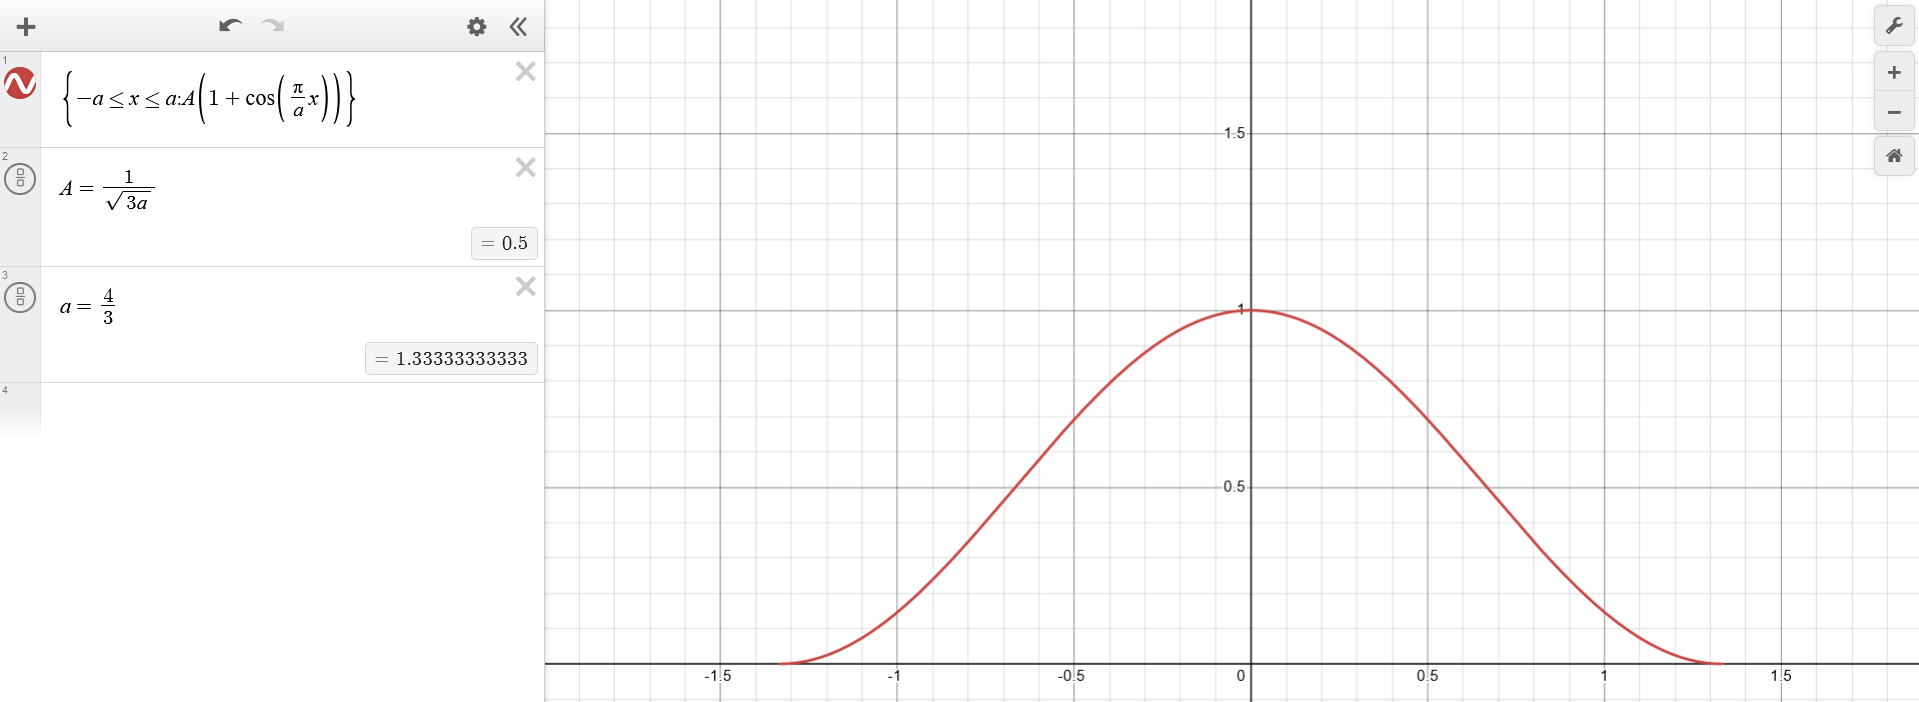
\includegraphics[width=0.7\linewidth]{Q1.png}
    \caption{$\psi$}
\end{figure}

(b) The classically allowed region is:
\[
    [-a, a]
\]
since the wave function \(\psi(x) = 0\) outside this interval, meaning the classical particle cannot be found outside \([-a, a]\).
\newpage
\section{Problem 2}

\begin{enumerate}
    \item
          \[
              \psi(x, t) = \sin \left( \frac{n \pi}{a} x \right) e^{-i \omega t}
          \]



          \[
              \frac{-\hbar^2}{2m}
              \frac{\partial^2 \psi}{\partial x^2} + V(x) \psi = i\hbar \frac{\partial \psi}{\partial t}
          \]

          \begin{equation*}
              \begin{split}
                  V(x) \psi
                    & = \frac{\hbar^2}{2m}
                  \frac{\partial^2 \psi}{\partial x^2}
                  + i\hbar \frac{\partial \psi}{\partial t}                                                                    \\
                    & = \frac{\hbar^2}{2m}
                  \frac{\partial^2 (\sin \left( \frac{n \pi}{a} x \right))}{\partial x^2}e^{-i \omega t}
                  + i\hbar \sin \left( \frac{n \pi}{a} x \right) \frac{\partial (e^{-i \omega t})}{\partial t}                 \\
                    & = - \frac{\hbar^2 n^2 \pi^2}{2ma^2} \sin\left( \frac{n \pi}{a} x \right) e^{-i \omega t}
                  + \omega \hbar \sin \left( \frac{n \pi}{a} x \right) e^{-i \omega t}                                         \\
                    & = (\omega \hbar - \frac{\hbar^2 n^2 \pi^2}{2ma^2}) \sin \left( \frac{n \pi}{a} x \right) e^{-i \omega t} \\
                    & = (\omega \hbar - \frac{\hbar^2 n^2 \pi^2}{2ma^2}) \psi                                                  \\
                  V & = \omega \hbar - \frac{\hbar^2 n^2 \pi^2}{2ma^2}
              \end{split}
          \end{equation*}

    \item

          To find the expectation value \(\langle x \rangle\), we observe that the term \(\sin^2 \left( \frac{n \pi}{a} x \right)\) is symmetric around \(x = \frac{a}{2}\). By shifting the domain of \(\psi(x)\) as \(\psi(x) \rightarrow \psi \left( x - \frac{a}{2} \right)\), we redefine the domain as \(-\frac{a}{2} \leq x \leq \frac{a}{2}\).

          Under this transformation, the shifted wave function becomes an even function, while \(x\) (as a variable) is odd with respect to \(x = 0\). As a result, the integrand for \(\langle x' \rangle = \int_{-\frac{a}{2}}^{\frac{a}{2}} x' |\psi(x')|^2 \, dx'\) is an odd function over a symmetric interval, leading to:

          \[
              \langle x' \rangle = 0.
          \]

          To obtain \(\langle x \rangle\) in the original coordinates, we perform the inverse transformation \(x' = x - \frac{a}{2}\), which implies \(x = x' + \frac{a}{2}\). Thus:

          \[
              \langle x \rangle = \langle x' + \frac{a}{2} \rangle = \langle x' \rangle + \frac{a}{2} = 0 + \frac{a}{2} = \frac{a}{2}.
          \]

          Therefore, the average position of the particle is:

          \[
              \langle x \rangle = \frac{a}{2}.
          \]

\end{enumerate}
\newpage
\section{Problem 3}
Fourier transform:
\[
    \phi(k) = \frac{1}{\sqrt{2\pi}} \int_{-\infty}^{\infty} \psi(x) e^{-ikx} \, dx
\]
Inverse Fourier transform:
\[
    \psi(x) = \frac{1}{\sqrt{2\pi}} \int_{-\infty}^{\infty} \phi(k) e^{ikx} \, dk
\]

\[
    \langle p \rangle = \int_{-\infty}^{\infty} \psi^*(x) \left( -i \hbar \frac{d}{dx} \right) \psi(x) \, dx
\]


\[
    \langle p \rangle = \int_{-\infty}^{\infty} \int_{-\infty}^{\infty} \phi^*(k') e^{-ik'x} \, dk' \left( -i \hbar \frac{d}{dx} \right) \int_{-\infty}^{\infty} \phi(k) e^{ikx} \, dk \, dx
\]

\[
    -i \hbar \frac{d}{dx} e^{ikx} = \hbar k e^{ikx}
\]
\[
    \langle p \rangle = \int_{-\infty}^{\infty} \int_{-\infty}^{\infty} \phi^*(k') \phi(k) \hbar k \left( \frac{1}{2\pi} \int_{-\infty}^{\infty} e^{i(k - k')x} \, dx \right) dk' \, dk
\]

\[
    \frac{1}{2\pi} \int_{-\infty}^{\infty} e^{i(k - k')x} \, dx = \delta(k - k')
\]

\[
    \langle p \rangle = \int_{-\infty}^{\infty} \int_{-\infty}^{\infty} \phi^*(k') \phi(k) \hbar k \delta(k - k')\, dk' \, dk
\]

\[ \therefore
    \langle p \rangle = \int_{-\infty}^{\infty} \hbar k |\phi(k)|^2 \, dk
\]

where \(|\phi(k)|^2\) represents the probability density in \(k\)-space and \(\hbar k\) is the momentum associated with each \(k\).

\newpage
\section{Problem 4}
\begin{enumerate}
    \item
          If a system is in a pure energy eigenstate, its time evolution is given by:

          \[
              \psi(x, t) = \psi(x, 0) e^{-i E t / \hbar}
          \]

          \[
              \psi(x, t + T) = \psi(x, t)
          \]

          \[
              \psi(x, 0) e^{-i E (t+T) / \hbar}  = \psi(x, 0) e^{-i E t / \hbar}
          \]

          \[
              \therefore e^{-i E T / \hbar} = 1
          \]

          \[
              \therefore \frac{E T}{\hbar} = 2 \pi n, \quad n \in \mathbb{N}
          \]

          \[
              T = \frac{2 \pi \hbar}{E} n
          \]

    \item

          \[
              E = \frac{2 \pi \hbar}{T} n
          \]

    \item
          For a particle in an infinite square well
          \[
              E_n = \frac{n^2 \pi^2 \hbar^2}{2m L^2}
          \]

          \[
              T = \frac{2 \pi \hbar}{E_n} n = \frac{4 m}{n \pi \hbar} L^2
          \]

\end{enumerate}

\newpage
\section{Problem 5}
The wave function stays undisturbed (the same) after the sudden expansion
\[
    \psi_0 = \sqrt{\frac{2}{L}}\cos{(\frac{\pi}{L}x)}, \quad -\frac{L}{2} \leq x \leq \frac{L}{2}
\]

% \begin{equation*}
%     \psi = 
%     \begin{cases}     
%         \sqrt{\frac{2}{L}}\cos{(\frac{\pi}{L}x)}, & , \quad \text{if} -\frac{L}{2} \leq x \leq \frac{L}{2} \\
%         0,& \text{otherwise}
%     \end{cases}
% \end{equation*}

The new ground state:

\[
    \psi'_0 = \sqrt{\frac{1}{L}}\cos{(\frac{\pi}{2L}x)}, \quad -L \leq x \leq L
\]

\begin{equation*}
    \begin{split}
        \langle \psi | \psi_0' \rangle
         & = \frac{\sqrt{2}}{L} \int_{-\frac{L}{2}}^{\frac{L}{2}} \cos{(\frac{\pi}{2L}x)}\cos{(\frac{\pi}{L}x)}\,dx                                        \\
         & = \frac{\sqrt{2}}{L} \int_{-\frac{L}{2}}^{\frac{L}{2}} \cos{(\frac{\pi}{2L}x)}[1-2\sin^2{(\frac{\pi}{2L}x)}]\,dx                                \\
         & = \frac{\sqrt{2}}{L} \left[\frac{2L}{\pi}\sin{(\frac{\pi}{2L}x)} - \frac{4L}{3\pi}\sin^3{(\frac{\pi}{2L}x)}\right]_{-\frac{L}{2}}^{\frac{L}{2}} \\
         & = \frac{2\sqrt{2}}{\pi} \left[\sin{(\frac{\pi}{2L}x)} - \frac{2}{3}\sin^3{(\frac{\pi}{2L}x)}\right]_{-\frac{L}{2}}^{\frac{L}{2}}                \\
         & =  \frac{8}{3 \pi}
        % & = \frac{2\sqrt{2}}{L} \int_{-\frac{L}{2}}^{\frac{L}{2}} \sin^2{(\frac{\pi}{2L}x)}\cos{(\frac{\pi}{2L}x)}\,dx \\
        % & = \frac{4\sqrt{2}}{3 \pi} \left[\sin^3{(\frac{\pi}{2L}x)}\right]_0^{L} = 0 = \frac{4\sqrt{2}}{3 \pi}
    \end{split}
\end{equation*}

\[
    P = |\langle \psi | \psi_0' \rangle|^2 = {|\frac{8}{3 \pi}|}^2 = \frac{64}{9\pi^2}
\]


\newpage
\section{Problem 6}



\newpage

\bibliographystyle{plain}
\bibliography{references}
\nocite{El-Deeb_PEU-323_Assignments}

\end{document}0^{L}